\documentclass{article}

\usepackage[margin=0.75in]{geometry}
\usepackage{graphics,graphicx}
\usepackage{parskip}
\usepackage{rotating}
\usepackage{tikz}
\usetikzlibrary{positioning,fit}

\usepackage{hyperref}
\hypersetup{
  colorlinks=true
}

\usepackage{fancyhdr}
\pagestyle{fancy}

\title{CBASS Design Document}
\author{David Carlson \and Sam Flint \and Kaleb Gaar \and Hayden Pollmann}

\begin{document}

\maketitle
\hypersetup{linkcolor=black}
\tableofcontents
\listoffigures
\hypersetup{linkcolor=red}

\section{Introduction}
\label{sec:introduction}

The goal of this document is to present the high-level architecture
and module relationships for CBASS, the Constraint-Based Anonymizable
Survey System.  It will include architecture and entity-relationship
diagrams to show the various relationships between different parts of
the system and the relationships within the database.  The primary
audience of the document is the various developers that will be
implementing and maintaining the system described herein.

\section{Architecture}
\label{sec:architecture}

\subsection{Introduction}
\label{sec:arch-introduction}

At a high-level, the overall design is a blend of both the repository
model and the Model-View-Controller paradigm.  In all situations, the
repository, or common database (\S\ref{sec:database}), accessed with a
common interface (\S\ref{sec:data-access-module}) is the model.  There
are three main controllers (\S\ref{sec:survey-designer},
\S\ref{sec:survey-taking} \& \S\ref{sec:surv-data-retr}), written in
Python, with corresponding views (\S\ref{sec:surv-design-interf})
implemented with HTML, CSS and Vue.JS.

\begin{figure}

  \begin{center}
    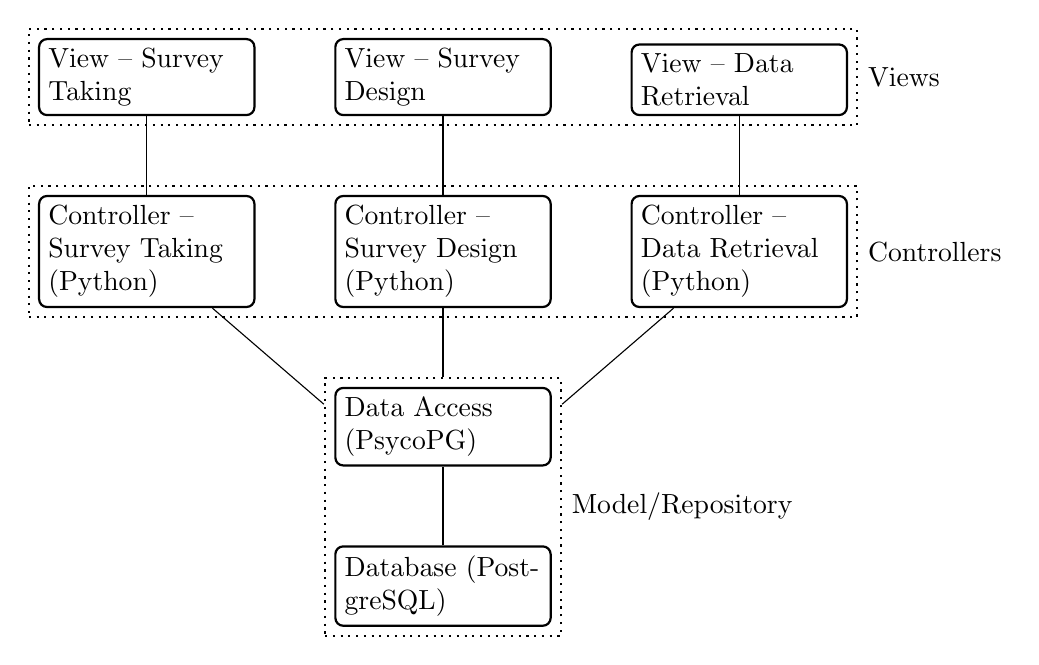
\begin{tikzpicture}[node/.style={rectangle, rounded corners=1mm, minimum size = 6mm, thick, draw, text width = 2.5cm}, default/.style={rectangle, rounded corners = 1mm, minimum size = 6mm, thick}, node distance = 10mm, box/.style={rectangle, minimum size = 10 mm, thick, draw, dotted}]
      \node [node] (db) {Database (PostgreSQL)};

      \node [node, above = of db] (da) {Data Access (PsycoPG)};

      \node [node, above = of da] (contDes) {Controller -- Survey Design\\ (Python)};

      \node [box, fit= (da) (db), label={right:Model/Repository}] (model) {};

      \node [node, left = of contDes] (contTake) {Controller -- Survey Taking (Python)};

      \node [node, right = of contDes] (contRetr) {Controller -- Data Retrieval (Python)};

      \node [box, fit= (contDes) (contTake) (contRetr), label={right:Controllers}] {};

      \node [node, above = of contDes] (viewDes) {View -- Survey Design};

      \node [node, above = of contTake] (viewTake) {View -- Survey Taking};

      \node [node, above = of contRetr] (viewRetr) {View -- Data Retrieval};

      \node [box, fit= (viewDes) (viewTake) (viewRetr), label={right:Views}] {};

      \path[-] (db) edge (da);

      \path[-] (model) edge (contDes);

      \path[-] (contDes) edge (viewDes);

      \path[-] (model) edge (contRetr);

      \path[-] (contRetr) edge (viewRetr);

      \path[-] (model) edge (contTake);

      \path[-] (contTake) edge (viewTake);
    \end{tikzpicture}
  \end{center}

  \caption{Overall Architecture}
  \label{fig:overall-arch}
\end{figure}

\subsection{Modules}
\label{sec:modules}

\subsubsection{Database}
\label{sec:database}

The Database is the key to the entirety of the CBASS, as it is the
repository where user data, survey data, and survey response data is
collected and stored until needed for use by the creator of the
survey.  It will run on PostgreSQL.  The database will contain many
relational tables for the storing of data
(\S\ref{sec:database-design}).  Controllers will access different
parts of the database through the Data Access Module.

\subsubsection{Data Access Module}
\label{sec:data-access-module}

Another important part of the system, the Data Access Module is
required for any part of the system to access data stored in the
Database.  It will achieve its functionality through the PsycoPG adapter
for PostgreSQL Databases.  The Data Access Module is an in-between that
communicates between the Controllers and the Database, taking commands
and retrieving, updating, or deleting respective data.

\subsubsection{Survey Designer Controller}
\label{sec:survey-designer}

The Survey Designer Controller will be responsible for the sending of
survey design data.  The Controller will accept input from the
Survey Design Interface (\S\ref{sec:surv-design-interf}) and will send create, update, and
delete commands to the Data Access Module (\S\ref{sec:data-access-module}).

\paragraph{Create}
\label{sec:survey-designer-create}

The Controller will create a new survey with the name of the survey as
input from the Survery Design Interface (\S\ref{sec:surv-design-interf}).  The Author of the
survey will be the User's ID.  The Controller will then handle sending
the survey question creation commands.  the Survey ID will be the ID of the
Survey.  The Controller will accept question text and question type as
inputs.  The Controller will also handle the creation of question
responses for the given question.  The Survey ID and Question ID will
be populated by the question and the survey.  The description and the
value will be inputs from the Survery Design Interface.  The
Author may create question constraints for a specific question and
response.  The Controller will take in a question from ID, response
from ID, the type of constraint, and the question affected ID.  For all
create commands, the Controller will update the View once the creation
has completed.

\paragraph{Update}
\label{sec:survey-designer-update}

The Controller will handle updating of a non-published survey.  A
survey may not be updated once it has been published.  The Author of
the survey may change the name of the survey.  The update command will
be sent to the Data Access Module (\S\ref{sec:data-access-module}) with inputs of the
Survey ID and the new Survey Name from the
Survery Design Interface (\S\ref{sec:surv-design-interf}).  The Author may change a survey
question text.  The update command will be sent to the
Data Access Module with inputs of the question ID and the
new question text.  The Author may change a question response
description.  The update command will be sent to the
Data Access Module with inputs of the question response ID
and the new response description.  For all update commands, the
Controller will update the View once the update has completed.

\paragraph{Delete}
\label{sec:survey-designer-delete}

The Controller will handle deletion of a survey.  A survey can only be
deleted if it is 1) nonpublished or 2) no responses have been recorded.
If responses to a survey have been entered, then the Survey data must be
kept in order to comply with Research Data Retention Best Practices.  The
delete command will be sent to the Data Access Module (\S\ref{sec:data-access-module}) with the
input of the Survey ID.  The Author of the survey may delete a survey
question.  The Controller will send a delete command with the question
ID as an input.  The Author of the survey may delete a question
response.  The delete command will be sent with the question response
ID as input, any question constraints tied to the question will also
be deleted.  The Author may delete a question constraint.  The
Controller will take a question constraint ID as input and send the
delete command.  For all delete commands, the Controller will update
the View once the deletion has completed.

\subsubsection{Survey Taking Controller}
\label{sec:survey-taking}

The Survey Taking Controller will be responsible for the sending of a
survey answer.  The Controller will accept input from the
Survey Taking Interface (\S\ref{sec:surv-taking-interf}) and send the create command to the
Data Access Module (\S\ref{sec:data-access-module}).  The Controller will send a
survey response entry create command composed of a survey
question ID, a question response ID, \& the response value.

The Controller will then query the database via the
Data Access Module to see what the next question in the
survey is.  Once the Controller has recieved the next question
information the View will be updated to the next question in the
Survey.

\subsubsection{Survey Data Retrieval Controller}
\label{sec:surv-data-retr}

The Survey Data Retrieval Controller will be responsible for the
retrieval and exportation of specific survey data pertaining to a
specific user.  The Controller will accept input from the
Survey Design Interface (\S\ref{sec:surv-design-interf}) and send the read commands to the
Data Access Module (\S\ref{sec:data-access-module}).  The Controller will accept The User's
ID and the ID of the Survey the User has selected.  Finally, The
Controller will update the View to show the survey data retrived.

The Controller will be responsible for data exportation.  The
Controller will take survey data as input and export the data to
either a CSV, Excel, JSON or SQL file.  The CSV exportation will be done
using standard Python file writting techniques.  The Excel exportation
will be done using the xlwt library.  The JSON exportation will done
using the standard json library.  The SQl exportation will be done
using a custom exportation process.  For all exportations the
Controller will update the View once the process has complete and give
a file availible for download to the User.

\subsubsection{Survey Interfaces}
\label{sec:surv-design-interf}

Users of the system will interact with the this level directly when
they design and take surveys.  Users will use this interface to login
into the survey system; view and edit surveys; and retrieve data from
survey responses.  This is also the layer of the system where
respondents will answer surveys.

The user interface will be composed of HTML, CSS, Javascript
(including the Vue library).  These technologies will create the
various components that represent the information received from the
controller.  This interface can be broken up into three major
components.

\paragraph{Survey Taking Interface}
\label{sec:surv-taking-interf}

This is the interface shown to a respondent when they are taking a
survey.  As questions are given and answered, only one will be present
on the screen at any given time.  Respondents will also be able to go
back to answer a previous question.

This interface will have a simple visual design, to aid readability
and decrease potential confusion in questions asked.  This feature
will be a key component of the initial implementation phase.

\paragraph{Survey Editing Interface}
\label{sec:surv-edit-interf}

The editing interface will allow users to create new surveys and
change unpublished surveys.  A survey will be represented as blocks of
questions, each with several editable fields (such as questions and
possible answers).  Each question block can have constrains added to
them, which will allow users to impose constrains onto other
questions.

This interface will be more complex, allowing users to see all of the
information relevant to survey construction in one browser window.
The editing interface will be a key component of the second
implementation phase.

\paragraph{User Information Interface}
\label{sec:user-infor-interf}

The user information interface will allow users to login to their
accounts, view all created surveys, and export survey respondent
information, as well as a few other account based functionality.
Simple versions of this component of the interface will be created
during the first and second implementation phases, but the majority of
its functionality is planned for future implementation.

% \section{Class Diagrams}
% \label{sec:class-diagrams}

\section{Database Design}
\label{sec:database-design}

\begin{sidewaysfigure}
  \includegraphics[width=\textwidth,height=\textheight,keepaspectratio]{{{relationships.real.large}}}
  \caption{Database Schema}
  \label{fig:db-schema}
\end{sidewaysfigure}

\subsection{Tables}
\label{sec:db-tables}

The following tables will be used to store data (see
Figure~\ref{fig:db-schema}):

\begin{description}
\item[Users] Will be used to keep track of users who create, modify
  and retrieve data from surveys.
\item[Surveys] Will be used to keep track of certain specific survey
  meta-data, including name, id and author.
\item[Survey Properties] Will be used to store other (optional) survey
  meta-data, including such things as IRB approval numbers, start and
  end messages and CSS/image customization.
\item[Survey Question] Will be used to store first a question text, in
  relation to a survey, along with the type of question, either single
  answer, multi-answer or free-response.
\item[Survey Response] Will be used to store certain meta-data about a
  response to a survey.   It will have a response ID, the survey, and a
  unique identifier string (sessionID or other) to ensure that while a
  survey is administered responses to individual questions may be
  collected as one single response.
\item[Question Response] Will be used to store the possible reponses
  for a given question, i.e., answers a, b and c for question X.
\item[Long Form Response] Will be used to store long-form question
  responses, i.e., essay-style or free-response.
\item[Multi Response] Will be used to store multi-choice responses,
  i.e., pick 0 or more of the following a, b, c, d for a given
  question.
\item[Standard Response] Will be used to store a single response to a
  given question.
\item[Question Constraint] Will be used to store ``FORBIDS'' and
  ``REQUIRES'' question constraints.
\item[Question Modify] Will be used to store modifications to a
  question based on previous responses, i.e., remove ability to
  respond with c, d from possible responses a, b, c, d, e, f, g.
\end{description}

\subsection{Relation Descriptions}
\label{sec:relat-descr}

\begin{itemize}
\item One-to-many User, Survey
\item One-to-many Survey, Survey Properties
\item One-to-many Survey, Questions
\item One-to-many Question, Question Responses
\item One-to-many Survey, Survey Response
\item One-to-many Survey Response, (Long Form Response, Multi
  Response, Standard Response)
\item One-to-many Question Response, Standard Response
\item Many-to-many Question Response, Multi Response
\item Many-to-many Question Response, Question Constraint
\item Many-to-many Question, Question Constraint
\item Many-to-many Question Response, Modify Constraint
\item Many-to-many Question, Modify Constraint
\end{itemize}

\end{document}

%%% Local Variables:
%%% mode: latex
%%% TeX-master: t
%%% End:
